\subsubsection*{問題(1)}
振動数が$\omega$となるような3次元調和ポテンシャル中に閉じ込められたひとつの粒子のエネルギー準位はゼロ点振動の成分を無視して
\begin{align}
  \epsilon_{n_x,n_y,n_z}=(n_x+n_y+n_z)\hbar\omega
\end{align}
で与えられる.ここで$n_x,n_y,n_z\in\mathbb{N}$である.

ここでエネルギーが$\epsilon$以下の状態数$\Omega(\epsilon)$とエネルギー状態密度$D(\epsilon)$を求めよ.\\
\hrulefill
\subsubsection*{解答}
$n_x+n_y+n_z=n$を満たすのは下図の点である.ここで状態が密に存在しているならエネルギー$\epsilon=n\hbar\omega$以下の状態数は底面積$n^2/2$,高さ$n$の三角錐の体積になるので
状態数$\Omega(\epsilon)$は
\begin{align}
  \Omega(\epsilon)=\frac{1}{3}\cdot n\cdot\frac{n^2}{2}=\frac{1}{6}\left(\frac{\epsilon}{\hbar\omega}\right)^3
\end{align}
また状態密度$D(\epsilon)$は
\begin{align}
  D(\epsilon)=\frac{{\rm d}\Omega}{{\rm d}\epsilon}=\frac{\epsilon^2}{2\hbar^3\omega^3}
\end{align}
である.
\begin{figure}[hptb]
  \begin{center}
    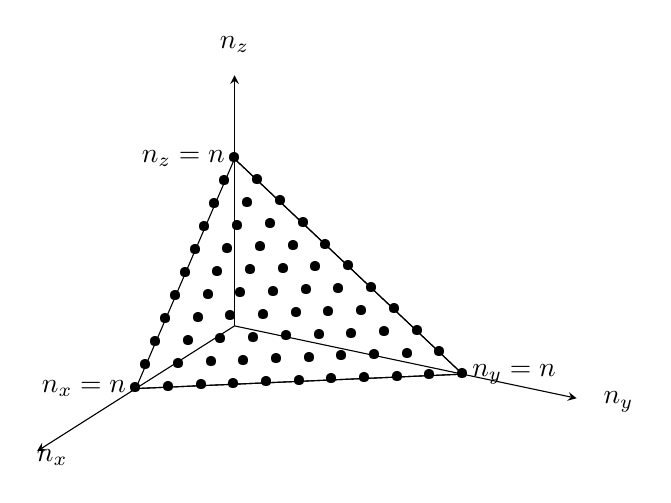
\begin{tikzpicture}[scale=1]
      \begin{axis}[
        view={120}{30},
        axis lines=center,
        ticks=none,
        xmin=0, xmax=20, ymin=0, ymax=15, zmin=0, zmax=15,
        xlabel=$n_x$, ylabel=$n_y$, zlabel=$n_z$,
        every axis x label/.style={
        at={(ticklabel* cs:1.05)},
        anchor=west,
        },
        every axis y label/.style={
        at={(ticklabel* cs:1.05)},
        anchor=west,
        },
        every axis z label/.style={
        at={(ticklabel* cs:1.05)},
        anchor=south,
        }
        ]
        %
        %\node at(axis cs:20,20,20) [anchor=west]{$\boldsymbol{n}$};
        %\draw[-stealth,red,very thick] (axis cs:10,10,10) -- (axis cs:20,20,20);
        \node at(axis cs:10,0,0) [anchor=east]{$n_x=n$};
        \node at(axis cs:0,10,0) [anchor=west]{$n_y=n$};
        \node at(axis cs:0,0,10) [anchor=east]{$n_z=n$};
        \draw[thin] (axis cs:10,0,0) -- (axis cs:0,10,0);
        \draw[thin] (axis cs:10,0,0) -- (axis cs:0,0,10);
        \draw[thin] (axis cs:0,10,0) -- (axis cs:0,0,10);
        \draw[thin] (axis cs:10,0,0) -- (axis cs:0,10,0) -- (axis cs:0,0,10);
        
        \node at (axis cs:10,0,0) {\textbullet};
        \node at (axis cs:9,1,0) {\textbullet};
        \node at (axis cs:8,2,0) {\textbullet};
        \node at (axis cs:7,3,0) {\textbullet};
        \node at (axis cs:6,4,0) {\textbullet};
        \node at (axis cs:5,5,0) {\textbullet};
        \node at (axis cs:4,6,0) {\textbullet};
        \node at (axis cs:3,7,0) {\textbullet};
        \node at (axis cs:2,8,0) {\textbullet};
        \node at (axis cs:1,9,0) {\textbullet};
        \node at (axis cs:0,10,0) {\textbullet};
        \node at (axis cs:9,0,1) {\textbullet};
        \node at (axis cs:8,1,1) {\textbullet};
        \node at (axis cs:7,2,1) {\textbullet};
        \node at (axis cs:6,3,1) {\textbullet};
        \node at (axis cs:5,4,1) {\textbullet};
        \node at (axis cs:4,5,1) {\textbullet};
        \node at (axis cs:3,6,1) {\textbullet};
        \node at (axis cs:2,7,1) {\textbullet};
        \node at (axis cs:1,8,1) {\textbullet};
        \node at (axis cs:0,9,1) {\textbullet};
        \node at (axis cs:8,0,2) {\textbullet};
        \node at (axis cs:7,1,2) {\textbullet};
        \node at (axis cs:6,2,2) {\textbullet};
        \node at (axis cs:5,3,2) {\textbullet};
        \node at (axis cs:4,4,2) {\textbullet};
        \node at (axis cs:3,5,2) {\textbullet};
        \node at (axis cs:2,6,2) {\textbullet};
        \node at (axis cs:1,7,2) {\textbullet};
        \node at (axis cs:0,8,2) {\textbullet};
        \node at (axis cs:7,0,3) {\textbullet};
        \node at (axis cs:6,1,3) {\textbullet};
        \node at (axis cs:5,2,3) {\textbullet};
        \node at (axis cs:4,3,3) {\textbullet};
        \node at (axis cs:3,4,3) {\textbullet};
        \node at (axis cs:2,5,3) {\textbullet};
        \node at (axis cs:1,6,3) {\textbullet};
        \node at (axis cs:0,7,3) {\textbullet};
        \node at (axis cs:6,0,4) {\textbullet};
        \node at (axis cs:5,1,4) {\textbullet};
        \node at (axis cs:4,2,4) {\textbullet};
        \node at (axis cs:3,3,4) {\textbullet};
        \node at (axis cs:2,4,4) {\textbullet};
        \node at (axis cs:1,5,4) {\textbullet};
        \node at (axis cs:0,6,4) {\textbullet};
        \node at (axis cs:5,0,5) {\textbullet};
        \node at (axis cs:4,1,5) {\textbullet};
        \node at (axis cs:3,2,5) {\textbullet};
        \node at (axis cs:2,3,5) {\textbullet};
        \node at (axis cs:1,4,5) {\textbullet};
        \node at (axis cs:0,5,5) {\textbullet};
        \node at (axis cs:4,0,6) {\textbullet};
        \node at (axis cs:3,1,6) {\textbullet};
        \node at (axis cs:2,2,6) {\textbullet};
        \node at (axis cs:1,3,6) {\textbullet};
        \node at (axis cs:0,4,6) {\textbullet};
        \node at (axis cs:3,0,7) {\textbullet};
        \node at (axis cs:2,1,7) {\textbullet};
        \node at (axis cs:1,2,7) {\textbullet};
        \node at (axis cs:0,3,7) {\textbullet};
        \node at (axis cs:2,0,8) {\textbullet};
        \node at (axis cs:1,1,8) {\textbullet};
        \node at (axis cs:0,2,8) {\textbullet};
        \node at (axis cs:1,0,9) {\textbullet};
        \node at (axis cs:0,1,9) {\textbullet};
        \node at (axis cs:0,0,10) {\textbullet};
      \end{axis}
    \end{tikzpicture}
  \end{center}
  \caption{$n_x+n_y+n_z=n$を満たす格子点}
  \label{fig:last}
\end{figure}